\section{Approximate Formulas}
%==========================================================
\subsection{sequential tunneling}
consider $T\simeq\mathit{\Delta}_{\mathrm{eff}}$\\
then the spectral function 
\begin{eqnarray}
	S(\omega)\equiv\frac{\mathrm{Im}[\chi(\omega)]}{\omega }
\end{eqnarray}
\begin{eqnarray}
	S(\omega) = \frac{\Delta}{\pi} \left[\delta(\omega-\Delta)+\delta(\omega+\Delta) \right]
\end{eqnarray}
is approximated as 
\begin{eqnarray}
	S(\omega)\simeq A\delta(\omega-\mathit{\Delta}_{\mathrm{eff}})+\delta(\omega+\mathit{\Delta}_{\mathrm{eff}})
\end{eqnarray}
where $\delta(x)$ is delta function.
then we apply  Kramers-Kronig relation
\begin{eqnarray}
	\frac{1}{\pi}\int_{-\infty}^{\infty}d\omega S(\omega)&=&\frac{1}{\pi}\int_{-\infty}^{\infty}d\omega \frac{\mathrm{Im}[\chi(\omega)]}{\omega}\\
&=&\mathrm{Re}[\chi (0)]
\end{eqnarray}
\begin{eqnarray}
	\chi_m \equiv \lim_{\epsilon \rightarrow 0} \frac{\langle \sigma_z \rangle}{\epsilon}
\end{eqnarray}
in the super ohmic and ohmic case $\chi_m=2\mathrm{tanh}(\beta \mathit{\Delta}_{\mathrm{eff}}/2)/\mathit{\Delta}_{\mathrm{eff}}$.
then  (\ref{exact_kappa}) is 
\begin{eqnarray}
	\kappa\simeq \frac{\pi\alpha\omega_c^{1-s}}{4}\frac{ \Delta_{\mathrm{eff}}^{s}}{2n(\Delta_{\mathrm{eff}})+1}\left[\frac{\beta\Delta_{\mathrm{eff}}/2}{\mathrm{sinh}{(\beta\Delta_{\mathrm{eff}}/2})}\right]^{2}
\end{eqnarray}
%==========================================================
\subsection{cotunneling}
consider lowtemperature $T\ll\mathit{\Delta}_{\mathrm{eff}}$, where $\mathit{\Delta}_{\mathrm{eff}}$is  abatically renormalized tunnneling rate.\\
generalized Shiba's relation
\begin{eqnarray}
	 \lim_{\omega \to 0+} \frac{\mathrm{Im}[\chi(\omega)]}{\omega^{s}}=2\pi\alpha\left(\frac{\chi_m}{2}\right)^{2}
\end{eqnarray}
where $\chi_m$ is susceptibility\\
then (\ref{exact_kappa}) is 
\begin{eqnarray}
	\kappa&\simeq& \frac{\pi\omega_c^{s-1}\chi_m^2}{8}\int_{0}^{\omega_{c}}d\omega  I_L(\omega)I_R (\omega)\left[\frac{\beta\omega/2}{\sinh{(\beta\omega/2)}}\right]^{2}
\end{eqnarray}
\begin{eqnarray}
	\kappa\simeq \frac{\pi\omega_c^{1-s}}{8}\left( \alpha \chi_m \right)^2 F(s)T^{2s+1}
	\label{cond_lowtemp},\\
	F (s)=\int_{0}^{\beta\omega_{c}}dx  x^{2s}\left[\frac{x/2}{\sinh({x/2})}\right]^{2}
\end{eqnarray}
%==========================================================
\subsection{incoherent  tunneling}
consider $T \gg \Gamma$. master eq.
\begin{eqnarray}
	\frac{dP_+(t)}{dt}=\Gamma P_-(t) - \Gamma P_+(t)
\end{eqnarray}
Fermi's golden rule
\begin{eqnarray}
	\Gamma&=&\left({\frac{\Delta}{2}}\right)^2\int_{-\infty}^{\infty}dt \ e^{-Q(t)},\label{Gamma} \\
		Q(t)&=&\int_{0}^{\infty}d\omega \frac{I(\omega)}{\omega^2}\left \{ \mathrm{coth\left(\frac{\beta \omega}{2}\right)[1-\mathrm{cos}(\omega t)]+\it{i} \ \mathrm{ sin}(\omega t)}\right \}
\end{eqnarray}
\begin{eqnarray}
	\langle\sigma_z(t)\rangle=\frac{P_+-P_-}{P_++P_-} =e^{-2\Gamma t}
	\label{sigma_z}
\end{eqnarray}
\begin{eqnarray}
	C(t)=\langle \sigma_z(t) \sigma_z(0) \rangle=e^{-2\Gamma|t|}  
\end{eqnarray}
\begin{eqnarray}
	C(t)&\equiv&\langle\sigma_z(t)\sigma_z(0)+\sigma_z(0)\sigma_z(t)\rangle/2\\
		&=&\langle \sigma_z(t) \sigma_z(0) \rangle\\
		&=&e^{-2\Gamma|t|}
\end{eqnarray}
Fourier transformation
\begin{eqnarray}
	C(\omega)=\frac{4\Gamma}{\omega^2+4 \Gamma^2}
\end{eqnarray}
fluctuation-dissipation theorem
\begin{eqnarray}
	 C(\omega)=\mathrm{coth}\left(\frac{\beta\omega}{2}\right)\mathrm{Im}[\chi(\omega)]
\end{eqnarray}
$T\gg\Delta$
\begin{eqnarray}
	C(\omega)&\simeq& 2\frac{\mathrm{Im}[\chi(\omega)]}{\beta \omega}=2TS(\omega)
\end{eqnarray}
then the spectral function is
\begin{eqnarray}
	S(\omega)=\frac{2\Gamma/T}{\omega^2+4\Gamma^2}\simeq \frac{2\Gamma}{\omega^2T}
\end{eqnarray}
then (\ref{exact_kappa}) is 
\begin{eqnarray}
	\kappa&\simeq&\frac{\alpha\omega_c^{1-s}}{4}\int_{0}^{\omega_c}d\omega \frac{2\Gamma}{T}\omega^{s-1}\left[\frac{\beta\omega/2}{\sinh{(\beta\omega/2)}}\right]^{2}\\
	&=&\frac{\alpha\omega_c^{1-s}}{2}G(s)\Gamma T^{s-1}	
\end{eqnarray}
\begin{eqnarray}
	G(s)=\int_{0}^{\beta \omega_c}dx\, x^{s-1}\left[\frac{x/2}{\sinh{(x/2)}}\right]^{2}
\end{eqnarray}
ohmic case
\begin{eqnarray}
	\kappa\simeq\frac{\sqrt{\pi}\Gamma(\alpha)}{4\Gamma(\alpha+1/2)}\frac{\Delta^2}{\omega_c}	\left(\frac{\pi T}{\omega_c}\right)^{2\alpha-1}
\end{eqnarray}
sub ohmic case
\begin{eqnarray}
	\kappa\simeq\frac{\alpha\omega_c^{1-s}}{2}G(s)\frac{\Delta^2}{4}e^{-\frac{\beta \Lambda_1}{4}}\sqrt{\frac{\pi \beta}{\Lambda_2}}T^{s-1} 
\end{eqnarray}
where
\begin{eqnarray}
	\Gamma&=&\frac{\Delta^2}{4}e^{-\frac{\beta \Lambda_1}{4}}\sqrt{\frac{\pi \beta}{\Lambda_2}},\\
	 \Lambda_1&=&8T\alpha\Gamma(s-1)+16T\alpha\Gamma(s-1)\left(\frac{T}{\omega_c}\right)^{s-1}(2-2^{s-1})\zeta(s-1),\\
	 \Lambda_2 &=&T\left(\frac{T}{\omega_c}\right)^{s-1}2\alpha(2^{s+1}-1)\Gamma(s+1)\zeta(s+1)
 \end{eqnarray}
\begin{figure}[tb]
 \centering
 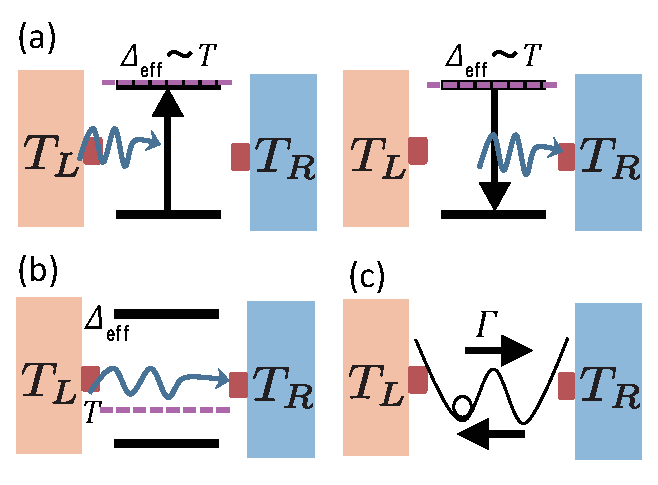
\includegraphics[width=100mm]{mechanism.eps}
 \caption{mechanism}
\end{figure}